\documentclass{article}
\usepackage{authblk}
\usepackage{hyperref}
\usepackage{inconsolata}
\usepackage[tt=false]{libertine}
\usepackage{graphicx}
\usepackage{indentfirst}

\begin{document}

\title{Computers, Sound, and Music: Project Report}
\author[]{Yuxiang Jiang}
\affil[]{\textit {yux@pdx.edu}}
\maketitle

\section{Introduction}

We present a real-time MIDI synthesizer in Rust, based on sample-based
synthesis techniques.
The synthesizer supports just one instrument which is a piano. The samples
that we use are from
\href{http://theremin.music.uiowa.edu/MIS.html}
  {The University of Iowa Musical Instrument Samples}. We preprocessed
the samples so that they sounds reasonable in our syntheized output.
We tested our synthesizer against many classical music MIDIs
from \href{http://www.piano-midi.de/}{piano-midi.de}.

\section{MIDI Format Overview}

A MIDI file consist of multiple tracks and each track contains a sequence
of events. The events consist of actual music notes,
control messages (e.g. instrument choice, damper pedal),
and meta messages (e.g. author name, tempo setting). The events
are timed -- each event occurs several `ticks` after the previous event.
This decides, e.g., the timing of the notes.

Our synthesizer only implements the minimal set of events that make playing
piano MIDI files possible:

\begin{itemize}
  \item \texttt{NoteOn(key, velocity)} marks the start of a music note.
    The key represents the pitch and the velocity represents the dynamics
    of the note. A 0 velocity means the same as a \texttt{NoteOff(key, \_)}

  \item \texttt{NoteOff(key, velocity)} marks the end of a music note.
    The velocity attribute represents the after-touch and is only used
    by some instruments (i.e., not for piano)

  \item \texttt{ProgramChange(instrument)} sets the instrument.
    A range of $[0,7]$ represents pianos.

  \item \texttt{ControlChange(which, value)} represents various instrument
    controls. For example, a `which` of 64 represents a damper pedal, where
    value $>= 64$ means on and otherwise off.

  \item \texttt{TempoSetting(microsPerBeat)} sets the tempo of the music.
\end{itemize}

\section{Preprocessing the Samples}

The piano samples from
\href{http://theremin.music.uiowa.edu/MIS.html}
  {The University of Iowa Musical Instrument Samples} are 44KHz stereo
  AIFF files. They are recorded with three dynamics: pp, mf, and ff.
  We wrote a Python script to download all the samples, and then analyzed
  their characterstics.

The below figures show the amplitudes of four mf notes, moving averaged
with a window size of 441 samples. The x axis represents the time (n-th
sample). The subfigure
titled `original` represents the files that are just downloaded. As can be seen
from the figure, the amplitude and the timing of the notes are very
different -- the attacks of different notes can be around 8000 samples apart
(which translates to a significant 0.2 seconds delay), and the amplitude
ratio between two samples can be as large as $200\%$. 
We synthesized some chords using the original samples and they sound horrible
-- it feels that the keys are not played at the same time.

We then came up with an automated way to normalize the samples, by
scaling their amplitudes and shifting the waves. Subfigure `scaled`
represents the samples that have their amplitude scaled linearly
and subfigure `shifted` represents the result of aligning the start of
the attacks. This turned out to be very effective -- synthesized chords
sounds like real chords now.

We save the normalized samples as FLAC files to keep them loseless. 

\begin{figure}[ht]
  \centering
  \includegraphics[page=1,width=\textwidth]{../norm/out.pdf}
  \caption{Amplitude Comparison}
\end{figure}

\section{Architecture of the Synthesizer}

We use Rust to write the synthesizer for its expressibility and performance.
Since our goal is to have real-time playback of MIDI files, it's crucial
that our synthesizer runs fast enough.

The core of our synthesizer is a MIDI event handler. It manages a list of the
notes that's currently being played, and accepts new MIDI events. When a new MIDI
event arrives after some interval, it elapses the current notes by several
ticks to generates samples, and then handles that new MIDI event. When a
\texttt{NoteOn(key, velocity)} occurs, we lookup the sample data using the key,
adjust the amplitude of the sample by the velocity, and add the resulting
sample data to the current note list.

To handle the damper pedal, we maintain the current state of the damper
pedal in our synthesizer. When a NoteOff occurs when the damper pedal
is on, we will keep playing that note. When the damper pedal is off while
there are still sustained notes playing, we will ramp down these notes in
a short time.

To meet the real-time goal, instead of batch generating all the samples
from a MIDI file at once, we instead interleave the synthesis of each event
and the sample playback. The synthesizer takes an array of MIDI events
and returns a (lazy) iterator of \texttt{f32} samples. As the playback
interface takes samples out of the iterator, the synthesizer consumes MIDI
events one by one, generating samples, until there are enough
samples to be played. This is achieved using unstable Rust's coroutine
feature, which allows us to write our synthesizer as a push-based stream.
The Rust compiler transforms the coroutine code into regular state machines
so that the coroutine code is platform independent.

\section{Evaluation}

We evaluated our synthesizer on our 2017 13-inch Macbook Pro with
7360U and builtin stereo speakers. We downloaded various
(Chopin, Mozart, Debussy, and Bach) piano MIDI files
from \href{http://www.piano-midi.de/}{piano-midi.de}, and compared our
synthesizer with MacOS's GarageBand's MIDI synthesizer.

\subsection{Feature Completeness}

Our synthesizer supports just enough MIDI event kinds to be able to play
the downloaded MIDI files.

\subsection{Sound Quality}

It's noticeable that our synthesizer produces lower-quality sounds. This
is partly due to the noise from the samples that we use. Our synthesizer
also sounds blurry while GarageBand sounds crispier. This is possibly
because that we handle different note dynamics by linearly mixing pp,
mf, and ff samples.

On the other hand, due to extensive use of envelopes in our synthesizer,
we at least are able to avoid most of the crackling sounds.

\subsection{Performance}

Our synthesizer takes around 6 seconds to synthesize Debussy's Clair De Lune.
And there's not much that we can do about that --
70\% of the time were spent in loading the piano samples, 10\% in synthesis,
and 20\% in writing to the output file.

Originally there was a bottleneck in the our synthesis engine\\
(\texttt{MidiSyn::\{syn,elapse\_notes\}} and \texttt{HashMap::insert})
and we fixed it by batch elapsing notes:

\begin{figure}[ht]
  \centering
  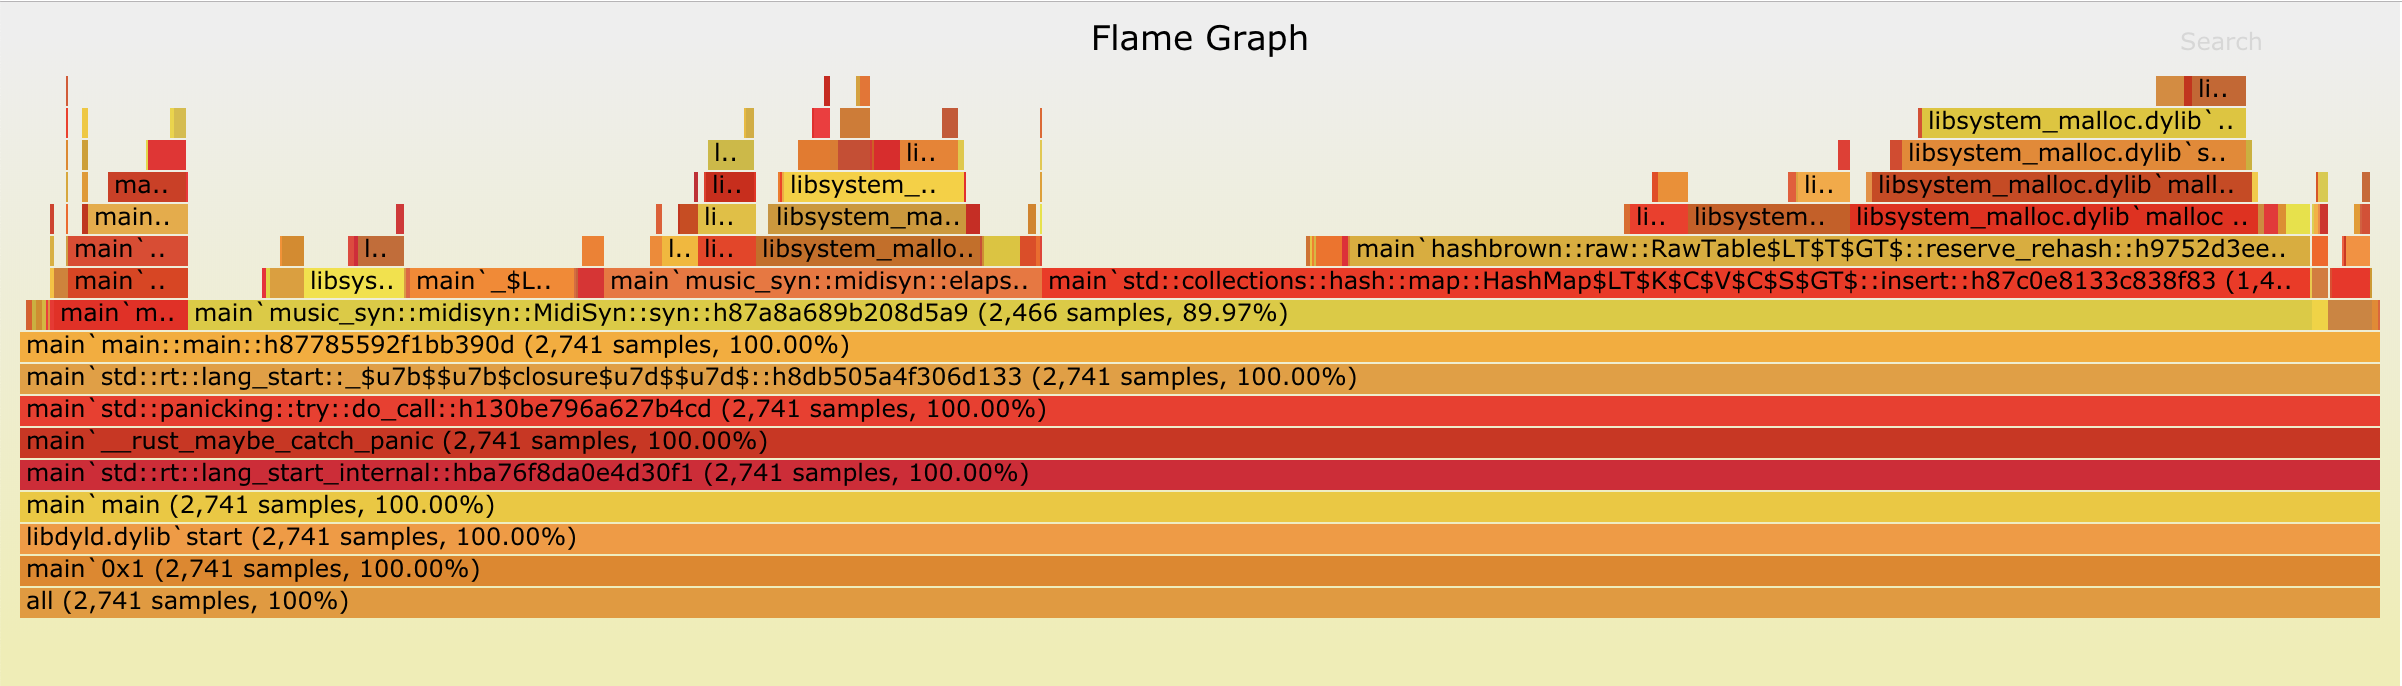
\includegraphics[page=1,width=\textwidth]{../perf/slow.png}
  \caption{Before Optimization}
\end{figure}

\begin{figure}[ht]
  \centering
  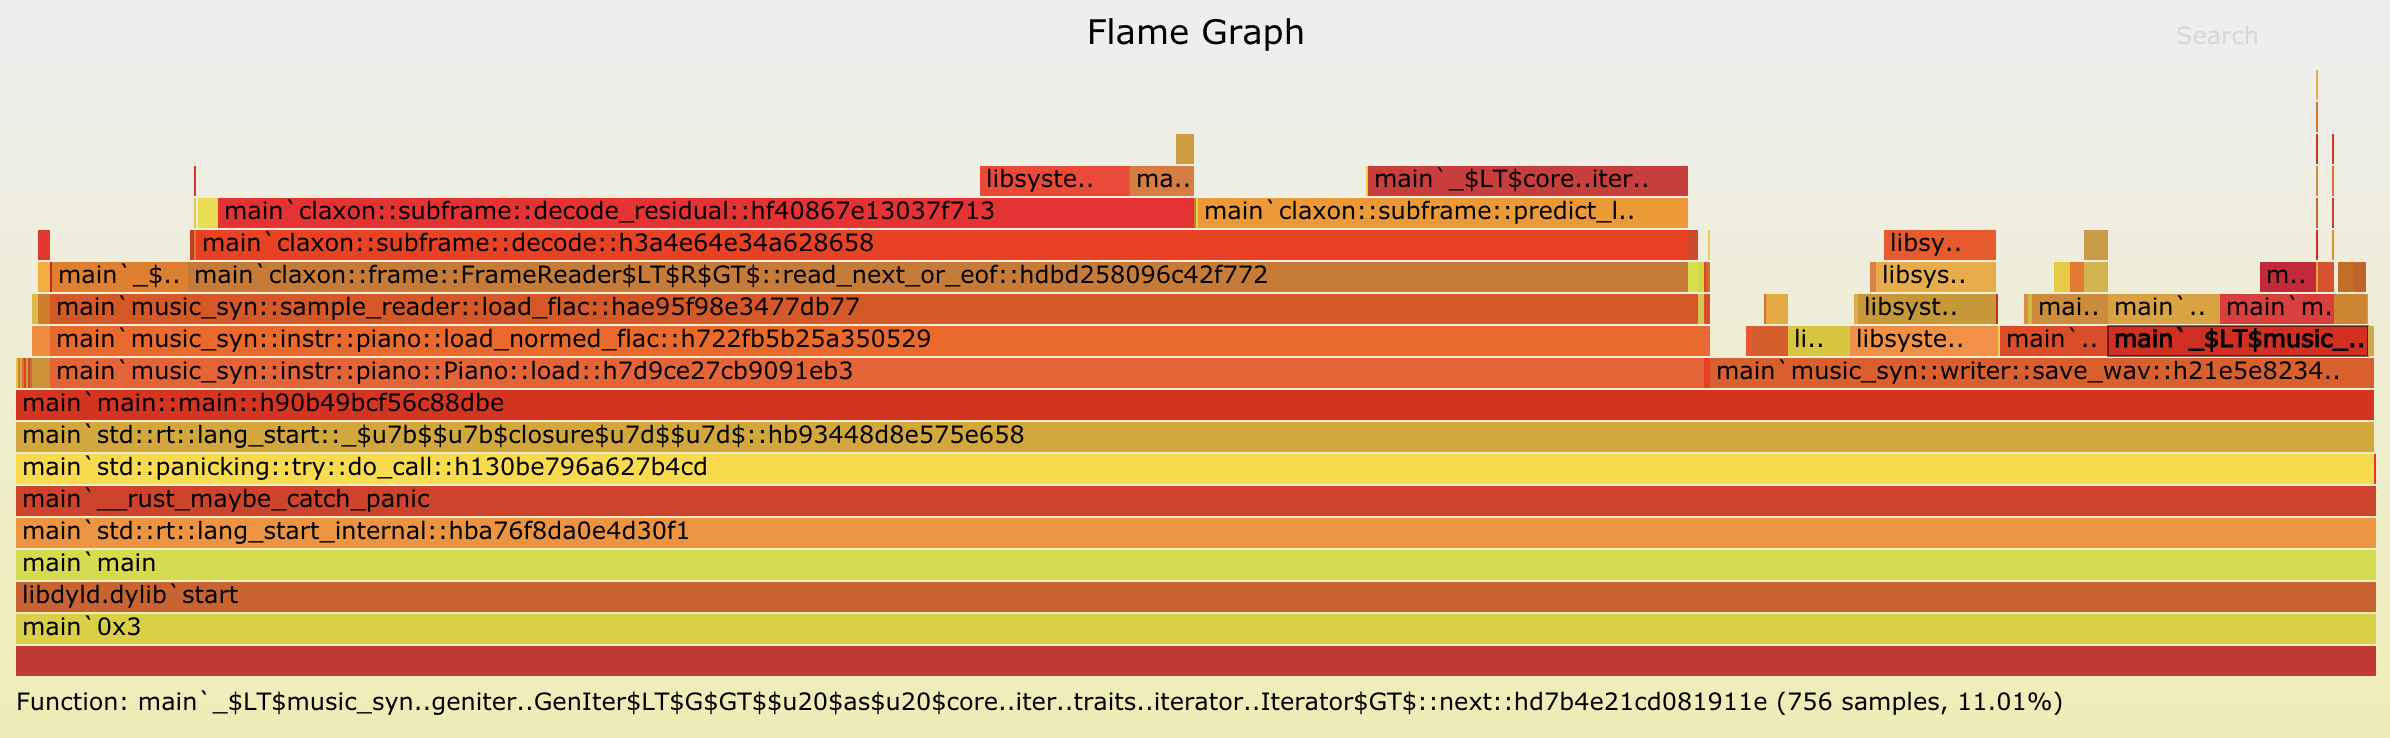
\includegraphics[page=1,width=\textwidth]{../perf/opt.png}
  \caption{After Optimization}
\end{figure}

\section{Limitations and Future Work}

Our synthesizer is certainly very incomplete feature wise.

\begin{description}
  \item [Other Instruments] We only have enough time to implement pianos.
    Other instruments suchs as guitars or organs might require more complex
    handling of the samples. For example, pressing an organ key produces
    a sustained sound which could possibly be infinite, while samples
    are always finite. This requires us to extract the sustained part from
    the samples and loop them.

  \item [Start-up Performance] At the start-up time, the synthesizer needs
    to load all 254 sample files (each around 1M in size) into the memory. This
    takes around 4 seconds on my 7360U laptop, which is a noticable delay. We can't
    think of a way to optimize this -- the Rust FLAC library we use is already
    as performant as libflac (which decodes faster than any other audio
    formats except for uncompressed PCM wav). Maybe we should collapse all
    the files into a whole to minimize syscalls? However syscalls don't
    seem to cost too much here...
    
  \item [Pull-Based Streaming] Currently we use a push-based approach for streaming
    synthesis. This works well in most of the cases, balancing the throughput
    and the latency. However, in the extremely case, one MIDI event could cause
    potentially huge number of samples to be synthesized, which causes lags.
    Switching to a pull-based streaming synthesis approach (i.e., instead of
    generating all samples from a given MIDI event at once, allows a MIDI event
    to be partially processed, so that the synthesizer can generate just enough
    samples that's reqested by the playback interface) would minimize
    latency.

  \item [GUI] It would be good to display an animated piano in the style
    of, e.g. Synthesia, during the playback. We will need to do a bit of
    lookahead when processing MIDI events to display the length of each
    animated note. And the graphics and the sound need to be synchronized.

  \item [Sequencer] Currently we only support MIDI format 0. In this format, there
    is only one track and every event happens in the track. To support
    multiple tracks, we will need to sequence the events before playing them.

  \item [Better Dynamics] Currently the piano dynamics are handled by
    linearly mixing pp, mf, and ff samples. This results in a blurry sound...
    Is there any better way to do this?
\end{description}

\section{Appendix}

\subsection{Running the Synthesizer}

The synthesizer requires portaudio and Rust nightly. Inside the
project root (e.g. the folder where Cargo.toml resides), run
\texttt{cargo run --release -- \$MIDI\_IN}
to play the given midi file, or
\texttt{cargo run --release -- \$MIDI\_IN \$WAV\_OUT}
to save the output to a file.

\subsection{Sample MIDI files}

\texttt{midi/} contains some sample MIDI files that's downloaded from 
\href{http://www.piano-midi.de/}{piano-midi.de}. See \texttt{midi/LICENSE}
for their license.

\subsection{Piano Samples}

We have already included the normalized piano sample files in the git repo
so you don't have to download and process them by yourself. But if you would
like to do that, please see \texttt{samples/} and \texttt{norm/pg.py} for
more details.

\end{document}
